\SourceLeaf{280}%
\Needspace{5\baselineskip}\begin{center}[3.]\end{center}

Interessant wird es in Beziehung auf diesen Gegenstand sein, zu
untersuchen 1) die Resultate des Durchschneidens der Knoten, in so fern
man

\begin{center}
\begin{minipage}{5.7cm}\centering statt:\quad\resizebox{2.4cm}{!}{%
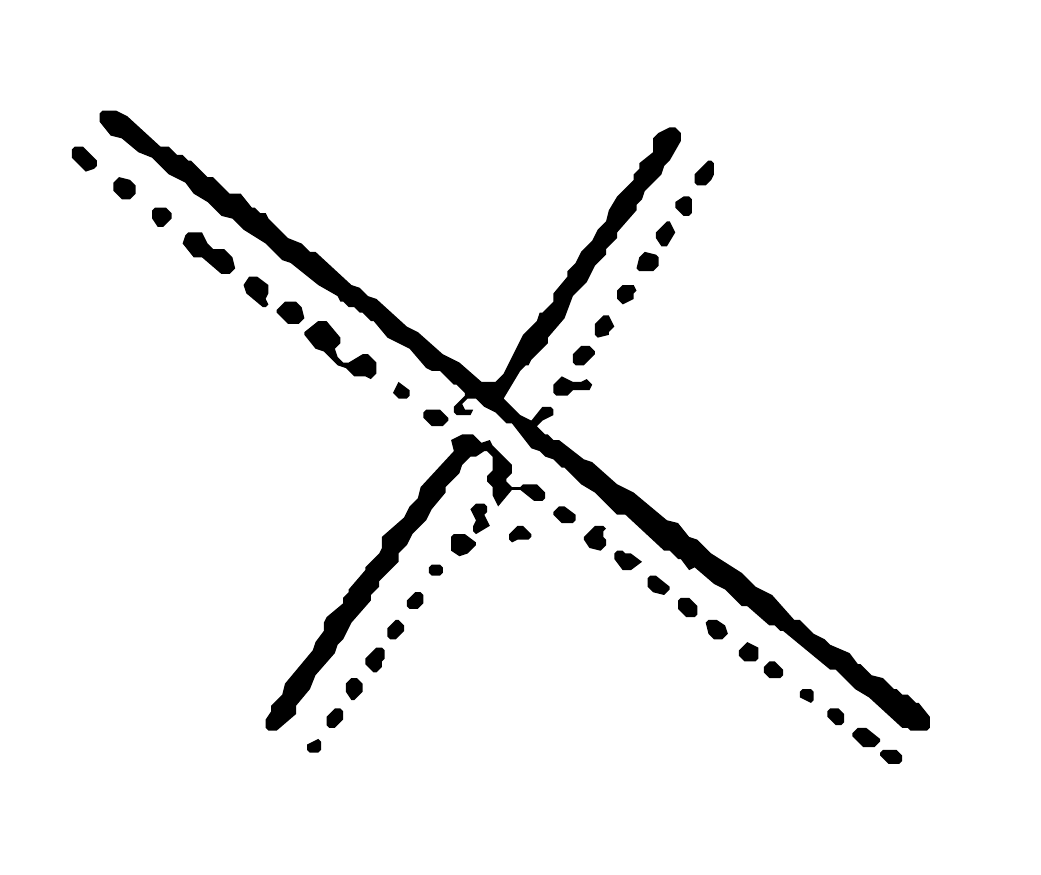
\begin{tikzpicture}[x=1pt,y=-1pt]
\path[use as bounding box] (0,0) rectangle (356,296);
\path[fill=black,draw=none,even odd rule]
(308,262) -- (308,263) -- (311,266) -- (315,266) -- (316,265) -- (316,263) -- (314,261) -- (309,261) -- cycle
(105,257) -- (101,259) -- (101,261) -- (102,262) -- (105,262) -- (106,261) -- (106,258) -- cycle
(298,255) -- (298,256) -- (302,260) -- (306,260) -- (308,258) -- (308,257) -- (303,253) -- (300,253) -- cycle
(290,246) -- (289,247) -- (289,249) -- (292,252) -- (294,252) -- (295,251) -- (295,248) -- (293,246) -- cycle
(113,246) -- (111,246) -- (108,249) -- (108,252) -- (109,253) -- (111,253) -- (114,250) -- (114,247) -- cycle
(280,239) -- (279,240) -- (279,242) -- (283,244) -- (284,243) -- (284,240) -- (283,239) -- cycle
(119,235) -- (117,235) -- (115,237) -- (115,240) -- (117,243) -- (118,243) -- (121,240) -- (121,237) -- cycle
(268,229) -- (266,231) -- (266,233) -- (268,235) -- (272,235) -- (273,234) -- (273,232) -- (270,229) -- cycle
(128,224) -- (126,224) -- (122,228) -- (122,230) -- (125,233) -- (126,233) -- (128,231) -- (128,229) -- (129,228) -- (129,225) -- cycle
(260,222) -- (257,225) -- (257,227) -- (259,229) -- (263,229) -- (264,228) -- (264,224) -- cycle
(246,214) -- (245,215) -- (246,219) -- (248,221) -- (251,221) -- (253,219) -- (252,216) -- (249,214) -- cycle
(134,214) -- (133,214) -- (130,217) -- (130,220) -- (131,221) -- (133,221) -- (136,218) -- (136,216) -- cycle
(236,206) -- (235,207) -- (235,210) -- (238,213) -- (241,213) -- (242,212) -- (242,209) -- (239,206) -- cycle
(142,204) -- (140,204) -- (137,207) -- (137,209) -- (138,210) -- (141,210) -- (143,208) -- (143,205) -- cycle
(225,198) -- (224,199) -- (224,202) -- (226,204) -- (230,205) -- (232,203) -- (232,202) -- (227,198) -- cycle
(146,194) -- (145,195) -- (145,197) -- (146,198) -- (149,198) -- (150,197) -- (150,195) -- (149,194) -- cycle
(212,190) -- (212,192) -- (215,196) -- (218,196) -- (222,193) -- (218,190) -- (216,190) -- (215,189) -- (213,189) -- cycle
(153,184) -- (153,189) -- (156,191) -- (159,190) -- (162,187) -- (162,186) -- (158,183) -- (154,183) -- cycle
(205,180) -- (201,184) -- (201,185) -- (203,188) -- (207,189) -- (209,187) -- (209,185) -- (208,184) -- (208,182) -- (209,181) -- (208,180) -- cycle
(174,183) -- (174,185) -- (175,186) -- (177,185) -- (181,185) -- (182,184) -- (182,183) -- (179,180) -- (177,180) -- cycle
(190,175) -- (190,176) -- (193,179) -- (197,179) -- (198,178) -- (198,176) -- (194,173) -- (192,173) -- cycle
(165,172) -- (162,172) -- (160,174) -- (162,178) -- (161,180) -- (161,182) -- (162,183) -- (167,180) -- (165,176) -- (166,175) -- (166,173) -- cycle
(167,149) -- (164,150) -- (161,147) -- (157,147) -- (153,149) -- (154,153) -- (142,166) -- (141,170) -- (138,173) -- (136,177) -- (128,184) -- (128,188) -- (127,190) -- (122,195) -- (122,196) -- (116,203) -- (116,204) -- (114,206) -- (114,208) -- (108,213) -- (107,215) -- (107,218) -- (104,222) -- (103,225) -- (93,237) -- (92,241) -- (88,245) -- (88,247) -- (86,250) -- (86,253) -- (87,254) -- (90,254) -- (97,248) -- (97,245) -- (102,239) -- (104,234) -- (111,226) -- (112,223) -- (114,221) -- (117,215) -- (124,207) -- (124,205) -- (127,202) -- (127,200) -- (134,193) -- (134,190) -- (137,187) -- (139,183) -- (144,178) -- (146,174) -- (151,168) -- (151,166) -- (156,161) -- (157,158) -- (160,155) -- (162,155) -- (165,153) -- (166,153) -- (168,155) -- (168,160) -- (166,162) -- (166,164) -- (168,166) -- (168,169) -- (170,173) -- (175,167) -- (178,167) -- (183,171) -- (186,171) -- (187,170) -- (187,168) -- (184,165) -- (179,165) -- (178,166) -- (175,166) -- (173,164) -- (173,163) -- (175,161) -- (175,158) -- (168,151) -- cycle
(143,139) -- (143,141) -- (146,144) -- (150,144) -- (152,142) -- (152,141) -- (149,138) -- (144,138) -- cycle
(134,128) -- (132,132) -- (134,134) -- (137,134) -- (138,133) -- (138,131) -- cycle
(190,132) -- (191,133) -- (195,133) -- (197,131) -- (203,131) -- (204,129) -- (202,127) -- (200,128) -- (197,128) -- (193,126) -- (190,129) -- cycle
(205,117) -- (203,115) -- (200,115) -- (197,118) -- (197,121) -- (198,122) -- (201,122) -- (205,118) -- cycle
(100,110) -- (100,111) -- (104,116) -- (107,117) -- (112,122) -- (115,123) -- (118,126) -- (122,126) -- (124,127) -- (126,125) -- (126,121) -- (123,118) -- (121,118) -- (116,121) -- (114,121) -- (112,119) -- (111,116) -- (113,114) -- (113,112) -- (108,106) -- (105,106) -- cycle
(210,104) -- (208,104) -- (205,107) -- (205,111) -- (206,112) -- (210,111) -- (210,110) -- (212,108) -- cycle
(93,99) -- (90,102) -- (90,103) -- (94,107) -- (98,107) -- (100,105) -- (99,101) -- (97,99) -- cycle
(219,93) -- (215,93) -- (213,95) -- (213,98) -- (215,100) -- (219,98) -- (219,96) -- (220,95) -- cycle
(80,90) -- (78,93) -- (79,96) -- (85,101) -- (86,101) -- (87,100) -- (86,98) -- (87,96) -- (87,93) -- (83,90) -- cycle
(223,81) -- (221,83) -- (220,87) -- (221,88) -- (226,88) -- (228,86) -- (228,83) -- (227,82) -- cycle
(57,75) -- (56,78) -- (60,83) -- (63,83) -- (70,89) -- (73,89) -- (75,87) -- (74,83) -- (71,80) -- (67,80) -- (65,78) -- (63,74) -- (58,74) -- cycle
(232,70) -- (231,70) -- (227,74) -- (227,76) -- (229,79) -- (231,79) -- (234,74) -- cycle
(46,65) -- (45,66) -- (45,69) -- (47,72) -- (49,72) -- (52,69) -- (52,67) -- (50,65) -- cycle
(237,61) -- (234,63) -- (234,65) -- (237,68) -- (239,68) -- (240,67) -- (240,62) -- (239,61) -- cycle
(33,54) -- (31,56) -- (31,59) -- (34,62) -- (37,62) -- (39,60) -- (39,57) -- (37,55) -- cycle
(247,48) -- (246,48) -- (241,53) -- (241,56) -- (242,57) -- (245,57) -- (247,55) -- (248,53) -- (248,49) -- cycle
(17,43) -- (16,44) -- (16,47) -- (21,52) -- (24,51) -- (25,50) -- (25,48) -- (20,43) -- cycle
(26,31) -- (26,34) -- (30,39) -- (34,40) -- (40,45) -- (45,47) -- (51,53) -- (57,56) -- (60,60) -- (65,63) -- (70,68) -- (74,69) -- (78,73) -- (86,78) -- (92,84) -- (95,85) -- (105,93) -- (112,97) -- (113,99) -- (114,99) -- (116,101) -- (118,101) -- (120,103) -- (121,103) -- (124,106) -- (125,106) -- (130,112) -- (138,116) -- (144,123) -- (146,124) -- (149,124) -- (154,129) -- (155,129) -- (158,132) -- (158,133) -- (154,137) -- (154,139) -- (155,140) -- (160,140) -- (161,138) -- (158,138) -- (157,136) -- (159,134) -- (162,134) -- (165,137) -- (169,139) -- (173,143) -- (175,143) -- (182,152) -- (185,153) -- (187,155) -- (190,156) -- (193,159) -- (194,159) -- (200,165) -- (205,168) -- (213,176) -- (216,176) -- (230,189) -- (232,189) -- (235,192) -- (236,192) -- (239,196) -- (241,195) -- (248,201) -- (252,203) -- (258,209) -- (260,209) -- (268,216) -- (270,216) -- (272,218) -- (273,218) -- (290,232) -- (292,232) -- (299,239) -- (304,242) -- (316,253) -- (318,253) -- (319,254) -- (325,254) -- (326,253) -- (326,249) -- (322,244) -- (321,244) -- (318,241) -- (316,241) -- (314,239) -- (313,239) -- (309,235) -- (305,234) -- (301,230) -- (300,230) -- (297,226) -- (290,223) -- (288,221) -- (284,219) -- (279,214) -- (277,214) -- (269,205) -- (263,202) -- (258,197) -- (247,190) -- (242,185) -- (239,184) -- (235,179) -- (231,178) -- (219,168) -- (213,165) -- (204,157) -- (201,156) -- (192,149) -- (190,149) -- (188,147) -- (187,147) -- (184,144) -- (186,142) -- (190,140) -- (190,138) -- (189,137) -- (186,137) -- (182,142) -- (178,140) -- (172,134) -- (178,124) -- (180,122) -- (181,122) -- (182,120) -- (188,114) -- (188,112) -- (194,105) -- (197,97) -- (202,92) -- (205,86) -- (209,82) -- (209,80) -- (213,76) -- (213,74) -- (220,66) -- (220,64) -- (222,62) -- (223,59) -- (229,53) -- (230,50) -- (232,48) -- (236,41) -- (236,38) -- (234,36) -- (232,36) -- (228,38) -- (226,40) -- (226,45) -- (221,49) -- (221,51) -- (219,53) -- (219,55) -- (213,61) -- (210,66) -- (209,70) -- (206,73) -- (204,77) -- (200,81) -- (198,85) -- (195,88) -- (195,90) -- (190,96) -- (190,99) -- (186,103) -- (185,103) -- (184,106) -- (179,111) -- (172,125) -- (169,128) -- (164,128) -- (156,121) -- (150,118) -- (141,110) -- (137,108) -- (126,98) -- (123,97) -- (120,94) -- (117,93) -- (104,81) -- (102,81) -- (99,78) -- (94,76) -- (87,69) -- (86,67) -- (84,67) -- (82,65) -- (81,65) -- (77,60) -- (73,60) -- (67,54) -- (65,54) -- (59,48) -- (58,48) -- (56,46) -- (54,46) -- (51,43) -- (48,43) -- (36,32) -- (32,30) -- (27,30) -- cycle;
\end{tikzpicture}%
}
\end{minipage}
\begin{minipage}{5.7cm}\centering setzt:\quad\resizebox{2.4cm}{!}{%
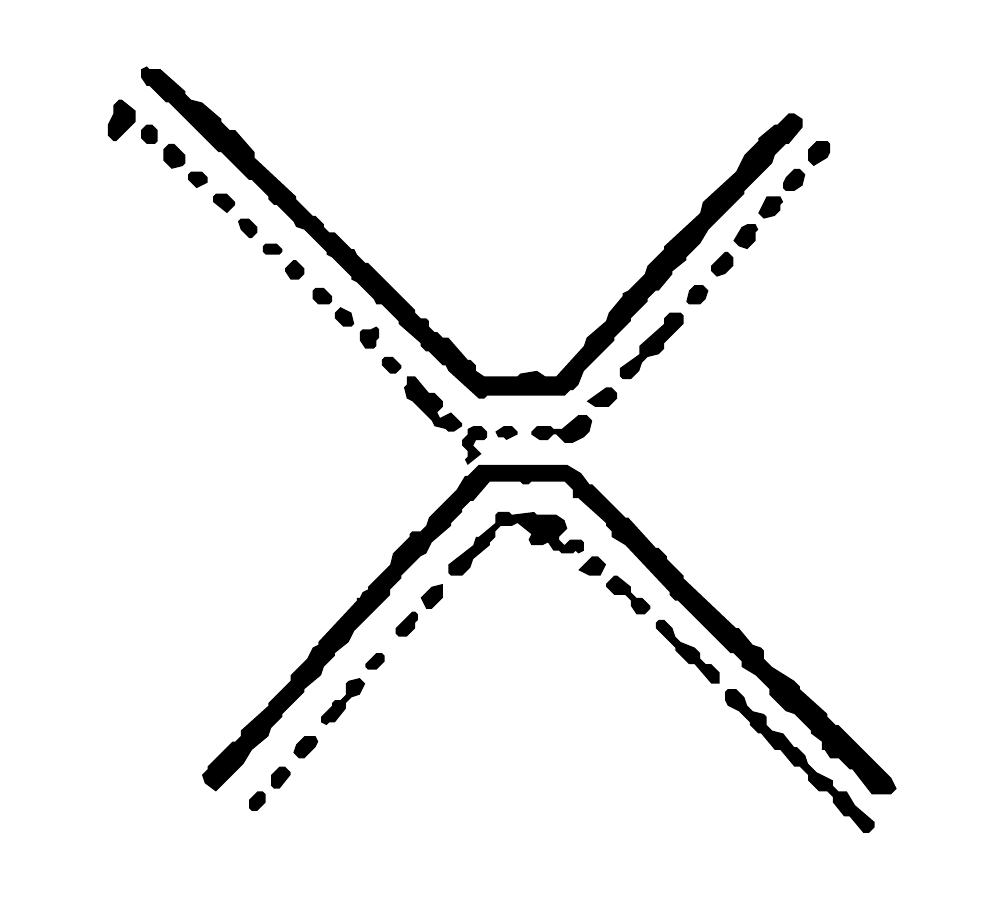
\begin{tikzpicture}[x=1pt,y=-1pt]
\path[use as bounding box] (0,0) rectangle (338,313);
\path[fill=black,draw=none,even odd rule]
(85,276) -- (83,276) -- (80,279) -- (80,282) -- (81,283) -- (83,283) -- (86,280) -- (86,277) -- cycle
(93,267) -- (91,267) -- (88,270) -- (88,274) -- (89,275) -- (91,275) -- (95,270) -- (95,269) -- cycle
(104,256) -- (100,256) -- (97,259) -- (96,262) -- (98,264) -- (100,264) -- (104,260) -- (105,258) -- cycle
(252,240) -- (252,243) -- (253,245) -- (257,247) -- (261,251) -- (261,252) -- (264,255) -- (265,255) -- (270,261) -- (272,261) -- (277,267) -- (279,267) -- (282,270) -- (282,272) -- (286,276) -- (289,276) -- (291,278) -- (291,280) -- (295,285) -- (297,285) -- (302,291) -- (304,291) -- (306,289) -- (306,287) -- (299,281) -- (296,276) -- (293,276) -- (291,274) -- (291,272) -- (285,269) -- (282,266) -- (281,263) -- (278,260) -- (277,260) -- (273,255) -- (269,254) -- (267,252) -- (267,249) -- (266,248) -- (262,247) -- (260,245) -- (259,242) -- (256,239) -- (253,239) -- cycle
(122,237) -- (120,235) -- (116,236) -- (115,237) -- (115,241) -- (113,243) -- (111,243) -- (110,244) -- (110,245) -- (106,249) -- (106,251) -- (108,252) -- (109,251) -- (111,251) -- (115,246) -- (115,244) -- (117,242) -- (120,241) -- cycle
(129,227) -- (128,226) -- (126,226) -- (122,230) -- (122,231) -- (123,232) -- (126,232) -- (129,229) -- cycle
(228,214) -- (227,215) -- (227,217) -- (234,224) -- (234,225) -- (239,230) -- (241,230) -- (247,237) -- (250,237) -- (250,233) -- (247,230) -- (245,230) -- (243,228) -- (243,226) -- (241,224) -- (236,222) -- (234,220) -- (233,217) -- (230,214) -- cycle
(140,211) -- (139,211) -- (133,217) -- (133,219) -- (134,220) -- (137,220) -- (140,217) -- (140,215) -- (141,214) -- (141,212) -- cycle
(150,201) -- (146,202) -- (142,206) -- (144,210) -- (146,210) -- (150,206) -- cycle
(212,198) -- (209,201) -- (209,202) -- (212,205) -- (216,205) -- (218,207) -- (218,209) -- (220,212) -- (223,212) -- (225,210) -- (225,209) -- (222,206) -- (220,206) -- (218,204) -- (218,202) -- (213,198) -- cycle
(199,196) -- (203,198) -- (207,198) -- (209,194) -- (206,191) -- (204,191) -- cycle
(152,197) -- (153,198) -- (157,198) -- (160,195) -- (161,192) -- (167,187) -- (167,186) -- (169,184) -- (169,182) -- (171,180) -- (175,180) -- (177,179) -- (182,183) -- (181,185) -- (182,187) -- (186,187) -- (188,186) -- (190,189) -- (192,189) -- (193,190) -- (197,190) -- (198,189) -- (199,190) -- (201,189) -- (201,186) -- (200,185) -- (196,185) -- (194,187) -- (192,185) -- (192,184) -- (195,181) -- (194,178) -- (191,176) -- (184,176) -- (183,175) -- (175,176) -- (174,175) -- (170,175) -- (169,176) -- (169,179) -- (163,184) -- (162,184) -- (161,187) -- (152,194) -- cycle
(63,270) -- (64,273) -- (68,276) -- (78,266) -- (81,261) -- (87,256) -- (88,253) -- (92,249) -- (92,248) -- (100,240) -- (100,239) -- (106,234) -- (107,231) -- (111,227) -- (111,226) -- (116,222) -- (118,218) -- (131,205) -- (131,203) -- (135,199) -- (135,198) -- (142,191) -- (144,190) -- (146,186) -- (153,180) -- (153,179) -- (157,175) -- (157,174) -- (160,171) -- (161,171) -- (167,164) -- (178,164) -- (179,165) -- (181,165) -- (182,164) -- (194,164) -- (197,167) -- (197,170) -- (199,170) -- (209,179) -- (209,180) -- (211,182) -- (211,184) -- (216,187) -- (232,204) -- (232,205) -- (234,207) -- (235,207) -- (254,226) -- (255,226) -- (258,229) -- (258,231) -- (263,234) -- (268,239) -- (268,241) -- (274,247) -- (277,248) -- (283,254) -- (283,255) -- (287,258) -- (287,261) -- (288,261) -- (290,264) -- (293,264) -- (297,268) -- (298,268) -- (305,277) -- (312,277) -- (314,275) -- (312,271) -- (293,252) -- (292,252) -- (289,249) -- (289,248) -- (279,239) -- (279,238) -- (277,236) -- (269,231) -- (266,228) -- (266,225) -- (265,224) -- (262,223) -- (257,217) -- (256,217) -- (237,199) -- (237,198) -- (231,192) -- (231,191) -- (228,188) -- (227,188) -- (217,177) -- (216,177) -- (204,165) -- (203,165) -- (200,161) -- (195,158) -- (163,158) -- (159,162) -- (158,162) -- (155,167) -- (145,177) -- (144,180) -- (142,182) -- (139,182) -- (138,183) -- (138,184) -- (132,190) -- (131,194) -- (123,202) -- (123,203) -- (121,204) -- (120,206) -- (119,206) -- (119,207) -- (105,222) -- (105,223) -- (103,224) -- (101,228) -- (95,234) -- (95,236) -- (87,244) -- (87,245) -- (77,254) -- (77,256) -- (75,258) -- (74,258) -- (65,267) -- (65,268) -- cycle
(169,146) -- (170,148) -- (172,148) -- (173,149) -- (177,147) -- (177,146) -- (175,144) -- (172,144) -- cycle
(164,144) -- (161,144) -- (159,145) -- (159,147) -- (157,149) -- (157,151) -- (159,153) -- (159,155) -- (158,156) -- (159,158) -- (164,154) -- (161,151) -- (162,149) -- (165,149) -- (166,148) -- (166,146) -- cycle
(204,142) -- (202,140) -- (199,140) -- (193,145) -- (190,145) -- (189,144) -- (184,144) -- (182,146) -- (182,147) -- (185,149) -- (188,149) -- (190,147) -- (191,147) -- (194,150) -- (197,150) -- (201,148) -- (203,146) -- cycle
(213,132) -- (211,130) -- (209,130) -- (202,135) -- (205,137) -- (210,137) -- (213,134) -- cycle
(137,126) -- (137,129) -- (136,130) -- (137,134) -- (139,135) -- (146,142) -- (147,144) -- (151,145) -- (152,146) -- (154,146) -- (157,144) -- (157,143) -- (153,139) -- (149,141) -- (148,139) -- (150,137) -- (150,135) -- (147,132) -- (145,132) -- (140,126) -- cycle
(129,119) -- (128,120) -- (128,122) -- (131,125) -- (133,125) -- (135,123) -- (135,122) -- (132,119) -- cycle
(126,108) -- (124,109) -- (121,109) -- (120,110) -- (120,113) -- (122,116) -- (125,116) -- (126,115) -- (126,113) -- (127,112) -- (127,109) -- cycle
(236,103) -- (232,103) -- (230,105) -- (230,107) -- (221,115) -- (221,118) -- (214,123) -- (214,126) -- (215,127) -- (218,127) -- (221,124) -- (222,121) -- (224,119) -- (228,118) -- (230,116) -- (230,114) -- (237,107) -- (237,104) -- cycle
(113,101) -- (111,103) -- (111,105) -- (114,108) -- (117,108) -- (118,107) -- (117,103) -- cycle
(104,94) -- (103,95) -- (103,98) -- (105,100) -- (109,100) -- (110,99) -- (110,97) -- (107,94) -- cycle
(246,95) -- (244,93) -- (241,93) -- (239,95) -- (238,99) -- (239,100) -- (243,100) -- (245,98) -- cycle
(96,84) -- (93,87) -- (93,88) -- (95,91) -- (98,91) -- (100,89) -- (100,87) -- (97,84) -- cycle
(253,81) -- (252,81) -- (247,86) -- (247,88) -- (249,90) -- (252,89) -- (255,86) -- (255,83) -- cycle
(85,79) -- (85,81) -- (86,82) -- (91,82) -- (92,81) -- (92,80) -- (90,78) -- (86,78) -- cycle
(263,71) -- (260,71) -- (258,72) -- (255,77) -- (257,79) -- (260,80) -- (263,77) -- (263,74) -- (264,73) -- cycle
(77,69) -- (76,70) -- (77,73) -- (80,76) -- (81,76) -- (83,74) -- (83,72) -- (80,69) -- cycle
(272,61) -- (267,61) -- (264,67) -- (266,69) -- (270,68) -- (272,66) -- (272,64) -- (273,63) -- cycle
(68,60) -- (67,61) -- (67,63) -- (72,67) -- (75,64) -- (75,63) -- (72,60) -- cycle
(58,53) -- (58,55) -- (61,58) -- (65,56) -- (65,54) -- (63,52) -- (59,52) -- cycle
(279,51) -- (277,51) -- (274,54) -- (273,56) -- (273,58) -- (274,59) -- (277,59) -- (280,57) -- (281,53) -- cycle
(51,42) -- (49,44) -- (49,48) -- (52,51) -- (56,50) -- (57,49) -- (57,46) -- (53,42) -- cycle
(289,41) -- (285,41) -- (282,44) -- (282,48) -- (284,50) -- (289,47) -- (290,45) -- (290,42) -- cycle
(43,35) -- (41,37) -- (41,40) -- (43,42) -- (46,42) -- (47,41) -- (47,37) -- (45,35) -- cycle
(34,26) -- (33,26) -- (31,28) -- (31,31) -- (29,35) -- (29,39) -- (31,41) -- (32,41) -- (39,34) -- (39,30) -- cycle
(41,15) -- (41,18) -- (43,21) -- (44,21) -- (50,27) -- (51,27) -- (69,45) -- (70,45) -- (80,55) -- (81,55) -- (87,61) -- (87,62) -- (89,64) -- (90,64) -- (96,70) -- (97,72) -- (100,73) -- (108,81) -- (108,82) -- (110,83) -- (117,90) -- (117,91) -- (119,92) -- (125,98) -- (126,100) -- (128,100) -- (134,106) -- (134,107) -- (142,114) -- (142,115) -- (144,117) -- (145,117) -- (150,122) -- (151,122) -- (152,124) -- (163,134) -- (165,134) -- (166,133) -- (194,133) -- (196,131) -- (197,131) -- (199,129) -- (201,124) -- (212,113) -- (212,112) -- (218,106) -- (218,105) -- (224,99) -- (224,98) -- (227,95) -- (228,95) -- (233,89) -- (233,88) -- (238,84) -- (238,83) -- (243,78) -- (246,73) -- (259,60) -- (259,59) -- (269,49) -- (270,46) -- (274,42) -- (275,42) -- (280,36) -- (280,33) -- (277,31) -- (275,31) -- (271,35) -- (270,35) -- (264,40) -- (264,41) -- (259,46) -- (256,52) -- (244,63) -- (243,67) -- (230,79) -- (230,80) -- (224,86) -- (223,89) -- (217,95) -- (215,96) -- (215,97) -- (210,103) -- (209,106) -- (202,112) -- (201,115) -- (191,126) -- (187,126) -- (184,124) -- (178,125) -- (177,126) -- (165,126) -- (162,124) -- (162,122) -- (160,120) -- (159,120) -- (152,112) -- (150,112) -- (148,110) -- (147,110) -- (145,108) -- (145,106) -- (144,105) -- (142,105) -- (140,103) -- (140,102) -- (123,85) -- (122,85) -- (119,82) -- (118,80) -- (117,80) -- (111,74) -- (109,74) -- (107,72) -- (107,71) -- (104,68) -- (103,68) -- (97,62) -- (97,61) -- (82,47) -- (82,45) -- (75,37) -- (73,37) -- (70,34) -- (70,33) -- (63,27) -- (59,26) -- (57,24) -- (57,23) -- (48,15) -- (44,15) -- (43,14) -- cycle;
\end{tikzpicture}%
}
\end{minipage}
\end{center}
\noindent wodurch dann lauter getrennte Grenzlinien entstehen. Zählt man dann für
jede Grenzlinie, die [die] $+$Seite innen hat, $+1$, und für
jede, die die $-$Seite innen hat, $-1$, so ist das Aggregat $\times 360^0$
die ganze Amplitudo. 

Vielleicht ist es fruchtbar, die Sache gleich anfangs noch allgemeiner
anzugreifen und mehrere Linien zugleich zu betrachten, deren jede in sich
selbst zurückkehrt, sich selbst und die andern
schneidet.

\Needspace{5\baselineskip}\begin{center}[4.]\end{center}

Das Vorhergehende ist richtig, verträgt aber grosse Vereinfachung. Indem
man die Linie durch die erwähnte Schneidung der Knoten in eine Anzahl in
sich zurückkehrender Linien theilt, die weder sich selbst noch einander
schneiden, braucht man nur anzugeben, gegen wie viele ($\mu$) Linien der
unendliche Raum auf der $-$Seite und gegen wie viele ($\nu$) auf der
$+$Seite liegt; man hat dann die Amplitudo

\[
= (\mu-\nu)\,360^0.
\]

Die Angabe ist aber leicht; da sogar die Relation jedes Punkts
angegeben werden kann. Es seien nemlich die Linien $a, b, c, d$
etc.\ und

\[
\frac{\partial(a)}{\partial a} = 0, \qquad \frac{\partial(a)}{\partial b} = \pm 1,
\]

je nachdem $a$ auf der $+$ oder $-$Seite von $b$ liegt, und so die
übrigen. Man hat dann, wenn in der ursprünglichen Figur der
Knoten vorkommt:

\[
\begin{array}{ccc}
x&&y \\
&n& \\
&\varepsilon,&
\end{array}
\]

\[
\frac{\partial y}{\partial x} = \varepsilon,
\]

\[
(y) - (x) = \varepsilon y + \varepsilon x,
\]
